\documentclass{article}
\usepackage{pgfplots}
\pgfplotsset{compat=1.18}

\begin{document}

\begin{figure}[h]
    \centering
    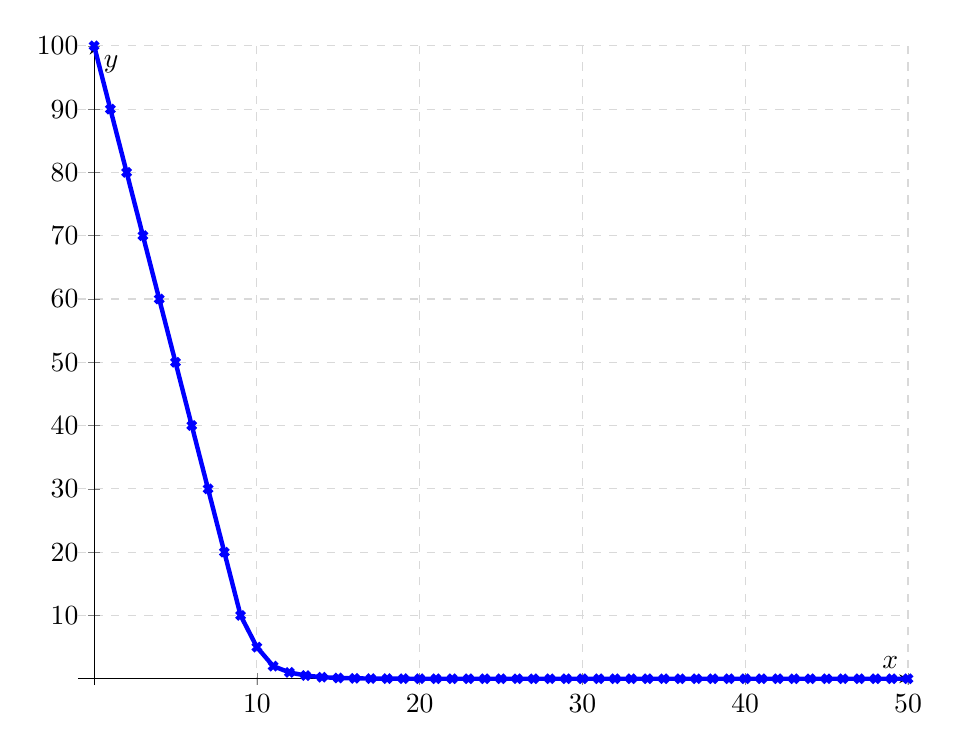
\begin{tikzpicture}
        \begin{axis}[
            width=\textwidth,
            height=0.8\textwidth,
            xlabel=$x$,
            ylabel=$y$,
            xmin=-1, xmax=50,
            ymin=-1, ymax=100,
            xtick={0,10,...,50},
            ytick={0,10,...,100},
            grid=major,
            grid style={dashed, gray!30},
            enlargelimits=false,
            clip=false,
            axis lines=middle,
            every axis plot/.append style={ultra thick},
            ]
            \addplot[blue, mark=x] coordinates {
                (0, 100)
                (1, 90)
                (2, 80)
                (3, 70)
                (4, 60)
                (5, 50)
                (6, 40)
                (7, 30)
                (8, 20)
                (9, 10)
                (10, 5)
                (11, 2)
                (12, 1)
                (13, 0.5)
                (14, 0.25)
                (15, 0.125)
                (16, 0.0625)
                (17, 0.03125)
                (18, 0.015625)
                (19, 0.0078125)
                (20, 0.00390625)
                (21, 0.001953125)
                (22, 0.0009765625)
                (23, 0.00048828125)
                (24, 0.000244140625)
                (25, 0.0001220703125)
                (26, 0.00006103515625)
                (27, 0.000030517578125)
                (28, 0.0000152587890625)
                (29, 0.00000762939453125)
                (30, 0.000003814697265625)
                (31, 0.0000019073486328125)
                (32, 0.00000095367431640625)
                (33, 0.000000476837158203125)
                (34, 0.0000002384185791015625)
                (35, 0.00000011920928955078125)
                (36, 0.000000059604644775390625)
                (37, 0.0000000298023223876953125)
                (38, 0.00000001490116119384765625)
                (39, 0.000000007450580596923828125)
                (40, 0.0000000037252902984619111328125)
                (41, 0.00000000186264514923095556640625)
                (42, 0.000000000931322574615477783203125)
                (43, 0.00000000046566128730773889160625)
                (44, 0.000000000232830643653869445803125)
                (45, 0.0000000001164153218269347229015625)
                (46, 0.00000000005820766091346736145078125)
                (47, 0.000000000029103830456733680725390625)
                (48, 0.00000000001455191522836684036265625)
                (49, 0.000000000007275957614183420181328125)
                (50, 0.0000000000036379788070917100906640625)
            };
        \end{axis}
    \end{tikzpicture}
    
    \begin{tikzpicture}
        \begin{axis}[
            width=\textwidth,
            height=0.8\textwidth,
            xlabel=$x$,
            ylabel=$y$,
            xmin=-1, xmax=50,
            ymin=-1, ymax=100,
            xtick={0,10,...,50},
            ytick={0,10,...,100},
            grid=major,
            grid style={dashed, gray!30},
            enlargelimits=false,
            clip=false,
            axis lines=middle,
            every axis plot/.append style={ultra thick},
            ]
            \addplot[green, mark=*] coordinates {
                (0, 0)
                (1, 2)
                (2, 4)
                (3, 8)
                (4, 16)
                (5, 32)
                (6, 64)
                (7, 128)
                (8, 256)
                (9, 512)
                (10, 1024)
                (11, 2048)
                (12, 4096)
                (13, 8192)
                (14, 16384)
                (15, 32768)
                (16, 65536)
                (17, 131072)
                (18, 262144)
                (19, 524288)
                (20, 1048576)
                (21, 2097152)
                (22, 4194304)
                (23, 8388608)
                (24, 16777216)
                (25, 33554432)
                (26, 67108864)
                (27, 134217728)
                (28, 268435456)
                (29, 536870912)
                (30, 1073741824)
                (31, 2147483648)
                (32, 4294967296)
                (33, 8589934592)
                (34, 17179869184)
                (35, 34359738368)
                (36, 68719476736)
                (37, 137438953472)
                (38, 274877906944)
                (39, 549755813888)
                (40, 1099511627776)
                (41, 2199023255552)
                (42, 4398046511104)
                (43, 8796093022208)
                (44, 17592186044416)
                (45, 35184372088832)
                (46, 70368744177664)
                (47, 140737488355328)
                (48, 281474976710656)
                (49, 562949953421312)
                (50, 1125899906842624)
            };
        \end{axis}
    \end{tikzpicture}
    
    \caption{The knot $o9\_{27767}$ has the Alexander polynomial $t^{130} - t^{129} + t^{121} - t^{120} + t^{114} - t^{113} + t^{111} - t^{110} + t^{105} - t^{104} + t^{102} - t^{101} + t^{98} - t^{97} + t^{95} - t^{94} + t^{92} - t^{91} + t^{89} - t^{88} + t^{86} - t^{85} + t^{83} - t^{82} + t^{81} - t^{80} + t^{79} - t^{78} + t^{76} - t^{75} + t^{73} - t^{71} + t^{70} - t^{69} + t^{67} - t^{66} + t^{65} - t^{64} + t^{63} - t^{61} + t^{60} - t^{59} + t^{57} - t^{55} + t^{54} - t^{52} + t^{51} - t^{50} + t^{49} - t^{48} + t^{47} - t^{45} + t^{44} - t^{42} + t^{41} - t^{39} + t^{38} - t^{36} + t^{35} - t^{33} + t^{32} - t^{29} + t^{28} - t^{26} + t^{25} - t^{20} + t^{19} - t^{17} + t^{16} - t^{10} + t^{9} - t + 1$ and $-3\int\Upsilon=15704/15$.}
\end{figure}

\end{document}